\documentclass[]{spie}

\renewcommand{\baselinestretch}{1.0}

\usepackage[utf8]{inputenc}
\usepackage{microtype}
\microtypesetup{expansion=false}
\usepackage{amsmath,amssymb}
\usepackage{booktabs}
\usepackage{graphicx}
\usepackage{xcolor}
\usepackage{tikz}
\usepackage{url}
\usepackage{xspace}
\usepackage{flafter}
\usepackage{placeins}
\usepackage[hidelinks]{hyperref}

\usetikzlibrary{arrows.meta,positioning,fit}

\newcommand{\method}{\textsc{DCTPR}\xspace}
\newcommand{\datasetcub}{CUB-200-2011\xspace}
\newcommand{\datasetdogs}{Stanford Dogs\xspace}

\title{DCTPR: Dual-capacity support-anchored refinement for low-latency high-way one-shot recognition}

\author[a]{Anonymous Author}
\affil[a]{Author names, affiliations, mailing addresses, and e-mail addresses
will be inserted before submission}
\authorinfo{Corresponding author information will be inserted before
submission.}

\pagestyle{empty}

\begin{document}
\maketitle

\begin{abstract}
Frozen visual foundation models provide strong transferable representations,
but one labeled image per class remains an unstable prototype in high-way
fine-grained recognition. Transductive solvers can correct this bias by using
the unlabeled query set, but iterative optimization can be costly. We present
Dual-Capacity Transductive Prototype Refinement (\method), a training-free task
adapter that fuses frozen DINOv2-B/14 and DINOv2-L/14 features, estimates
class-balanced query centers, and applies a short support-anchored update.
Across three 200-way CUB episodes and three 120-way Stanford Dogs episodes,
\method improves fused nearest-support accuracy by 6.68 and 6.27 percentage
points, respectively. It remains within 1.35 points of TIM-ADM on CUB and 0.61
points of MAP-RAW on Dogs, while its task head is 3.8 and 49 times faster than
those strongest matched solvers. Controlled imbalance tests show that the
result depends on a known balanced query prior. A locked official-test audit
preserves the same relative behavior without retuning. Under a 50-ms-per-rotation
task-head budget, it is the highest-accuracy method on both datasets among the
matched solvers. These results support a scoped low-latency state-of-the-art
claim under the matched frozen-feature protocol, not a global accuracy claim.
\end{abstract}

\keywords{few-shot learning, transductive inference, fine-grained recognition,
frozen visual foundation models, prototype refinement}

\section{Introduction}
\label{sec:introduction}

Fine-grained recognition asks a model to separate categories whose defining
differences may be smaller than changes in pose, viewpoint, background, or
within-class appearance. The problem becomes especially consequential when new
categories must be recognized from a single labeled example and no backbone
update is affordable. This paper studies that limit directly: reliable,
low-cost recognition of all 200 bird classes or all 120 dog breeds from one
support image per class, using frozen visual foundation models. The central
question is whether query-set structure can correct an unreliable one-shot
decision rule without replacing representation learning with another expensive
task-specific optimization stage.

This setting is difficult because one image must serve simultaneously as the
supervision signal and the class prototype. If that image has an atypical pose,
crop, or background, its embedding can be displaced from the query cluster;
high-way competition then magnifies even a small displacement among visually
similar classes. Attention, feature reconstruction, and cross-image
correspondence reduce related fine-grained ambiguities
\cite{mamlfgvc,dualattention,bfrn}, while transfer-based studies show that a
strong representation can make simple classifiers surprisingly competitive
\cite{closerlook,goodembedding,simpleshot}. Yet a stronger encoder does not by
itself turn one observation into a reliable estimate of the class center.
DINOv2 therefore improves the geometry available to the task head
\cite{dinov2}, but it does not remove the one-shot estimation problem.

Transductive inference can address this problem by estimating labels jointly
over the unlabeled query set. LaplacianShot exploits a query graph
\cite{laplacianshot}, TIM optimizes a mutual-information objective \cite{tim},
and PT-MAP alternates optimal-transport assignments with prototype updates
\cite{ptmap}. These approaches show that query geometry can correct
single-support bias, but graph construction or repeated optimization incurs
task-level latency. Their behavior can also depend strongly on the assumed
query-class proportions \cite{realistictransduction}. The remaining problem is
therefore not simply to maximize accuracy: it is to recover most of the useful
transductive correction with a short, transparent update whose computational
cost and query-prior boundary are both explicit.

We propose Dual-Capacity Transductive Prototype Refinement (\method) for this
purpose. Its design follows three observations. First, frozen DINOv2-B/14 and
DINOv2-L/14 embeddings provide distinct capacity views of the same episode, so
their normalized class-token features can be fused without task-specific
training. Second, when the episode construction guarantees equal queries per
class, a soft Sinkhorn assignment can express that known marginal while using
the entire query set to estimate class centers. Third, the labeled support
should remain an anchor rather than be discarded: mixing each estimated query
center with its original support limits prototype drift. Alternating assignment
and anchored updates for exactly three steps yields a gradient-free task adapter
that neither reads query labels nor learns task-specific parameters.

Experiments under a frozen development--confirmation protocol show how far this
compact update resolves the problem. Across CUB-200-2011 and Stanford Dogs,
\method improves fused nearest-support accuracy by 6.68 and 6.27 percentage
points. It remains 1.35 points below TIM-ADM on CUB and 0.61 points below
MAP-RAW on Dogs, while reducing task-head runtime by factors of 3.8 and 49,
respectively. A locked official-test audit preserves these relative conclusions,
and controlled imbalance tests identify the known balanced query marginal as a
real limitation. Thus the contribution is a specified accuracy--efficiency
operating point for balanced high-way one-shot recognition: a reproducible
dual-capacity adapter, a matched evaluation against established transductive
solvers, and an explicit audit of runtime and query-prior sensitivity. Within
the stated 50-ms task-head budget, it gives the highest accuracy in the tested
solver set on both datasets. Because stronger matched solvers retain higher
absolute accuracy outside that budget, this is a scoped low-latency state-of-
the-art claim rather than a global accuracy claim.

\section{Related Work}
\label{sec:related}

\subsection{Frozen representations for few-shot recognition}

Transfer-based few-shot learning often separates representation learning from
task inference. A strong encoder can make simple nearest-center or linear
classifiers competitive, which places a higher burden on any adaptation module
to show that its gain is not caused by a weak feature baseline
\cite{closerlook,goodembedding,simpleshot}. DINOv2 learns
general-purpose visual features through self-supervised pretraining
\cite{dinov2}. We therefore freeze both DINOv2 encoders in all experiments and
apply every compared transductive solver to the same extracted features. This
design isolates task inference from backbone optimization.

Fine-grained datasets add a complementary challenge: class identity can depend
on small appearance differences while nuisance variation dominates the image.
CUB \cite{cubdataset} and Stanford Dogs \cite{stanforddogs} are widely used to
study such distinctions, including in attention- and reconstruction-based
few-shot recognition \cite{mamlfgvc,dualattention,bfrn}. Rather than
constructing a conventional 5-way task,
we evaluate all available categories in each episode. This high-way setting
magnifies competition among similar categories and makes support-prototype bias
visible even with foundation-model features.

\subsection{Transductive inference and prototype correction}

Transductive methods use the query set jointly rather than predicting each query
independently. LaplacianShot optimizes unary support distances together with a
graph smoothness term \cite{laplacianshot}. TIM alternates classifier updates
under supervised support and query information objectives \cite{tim}. PT-MAP
applies a feature transform and Sinkhorn-based assignment before iteratively
moving class prototypes \cite{ptmap}. Related work also shows that careful
feature preprocessing and simple classifier ensembles can remain competitive
without episodic meta-training \cite{squeezefeatures,easy}. More recent work further combines graph
and prototype refinement \cite{iterativegraph} or learns conditional transport
for unknown query proportions \cite{conditionaltransport}.

The idea that a short correction can substantially improve one-shot prototypes
predates these iterative solvers. BDCSPN rectifies prototypes by shifting them
with pseudo-labeled query features in a small number of steps, explicitly
targeting intra-class bias from scarce supports \cite{bdcspn}. \method shares
that inexpensive-correction premise, and the comparison is therefore about what
is corrected rather than whether cheap correction is novel: BDCSPN rectifies
within one representation, whereas we anchor a class-balanced update across two
frozen capacities and characterize the resulting operating point against
iterative solvers. Recent work also reduces the hyper-parameter burden of these
objectives, either by removing tuned parameters altogether
\cite{paddle} or by unrolling the optimizer and learning its
hyper-parameters \cite{unem}. Our schedule is instead fixed by construction and
transferred across datasets without retuning, which trades attainable accuracy
for a predictable cost.

\method does not claim the individual novelty of feature concatenation,
Sinkhorn normalization, or prototype refinement; nor of cheap prototype
correction in general. Its contribution is the scoped
combination of complementary frozen capacities with a deliberately short update
schedule, together with a matched high-way accuracy--efficiency evaluation. The
method is consequently compared against the established solver families on the
same feature tensors instead of against a weaker classifier alone.

\subsection{Query priors in transductive evaluation}

Balanced query sets provide useful controlled evaluation, but they also reveal
the class marginal to the inference procedure. Veilleux et al. showed that
methods encoding a uniform marginal can degrade under Dirichlet-distributed
query proportions and proposed an alpha-entropy objective to reduce this bias
\cite{realistictransduction}. Conditional transport and adaptive-manifold
methods subsequently targeted imbalanced transduction directly
\cite{conditionaltransport,adaptivemanifold}, as did hyper-parameter-free and
unrolled formulations that do not presuppose a uniform marginal
\cite{paddle,unem}. We treat balance as an explicit
assumption rather than a hidden property. Our primary experiments test the
balanced high-way setting, while separate mild and severe imbalance regimes
measure how far the conclusion extends.

We do not compete with this line of work. Those methods are developed and
compared on the public 5-way protocol with Dirichlet-sampled query proportions,
whereas our episodes are high-way with deterministic class counts, so the
numbers are not commensurable. Our imbalance results are a scope boundary for
the proposed operating point, not a claim about imbalanced transduction; closing
that gap requires the public protocol and matched backbones, which we identify
as future work rather than a contribution of this paper.

\section{Method}
\label{sec:method}

\subsection{Task formulation}

An episode contains $C$ classes and one labeled support image per class,
$\mathcal{S}=\{(x_c^s,c)\}_{c=1}^{C}$. The unlabeled query set is
$\mathcal{Q}=\{x_i^q\}_{i=1}^{N}$. In the primary protocol, each class occurs
exactly $q=N/C$ times in $\mathcal{Q}$, but query labels are never observed by
the method. The goal is to predict all query labels jointly using frozen image
features and the known balanced column mass $q$.

Figure~\ref{fig:pipeline} summarizes \method. Two frozen encoders produce
complementary image representations. The fused support features initialize the
class prototypes. Each refinement step alternates a balanced soft assignment
with a support-anchored query-center update. The final assignment provides the
query predictions.

\begin{figure}[!htbp]
\centering
\resizebox{\textwidth}{!}{%
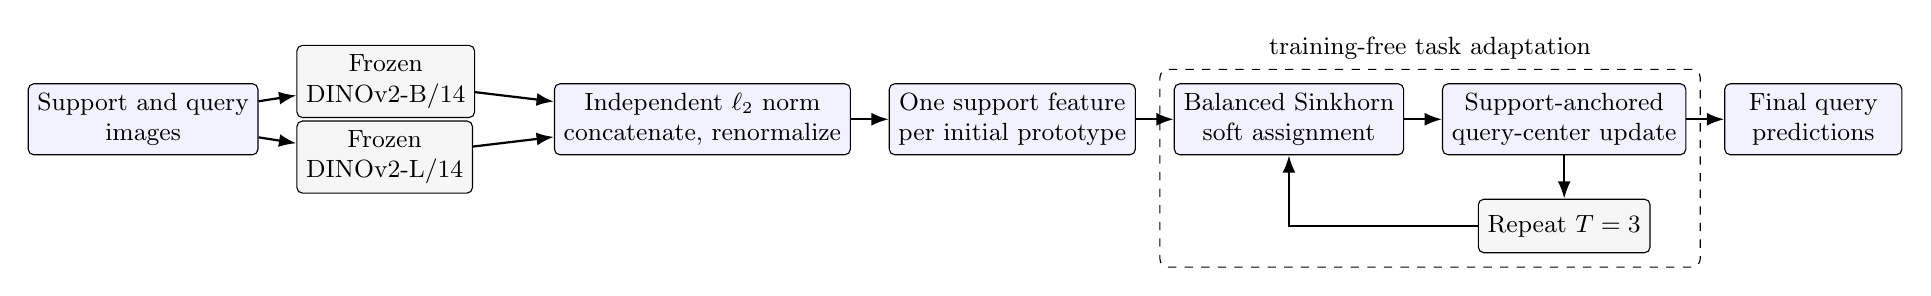
\begin{tikzpicture}[
  node distance=0.55cm and 0.48cm,
  block/.style={draw, rounded corners=2pt, align=center, minimum height=0.78cm,
                minimum width=2.25cm, fill=blue!5, font=\small},
  smallblock/.style={draw, rounded corners=2pt, align=center, minimum height=0.68cm,
                minimum width=1.95cm, fill=gray!7, font=\small},
  arrow/.style={-{Latex[length=2.2mm]}, thick},
  group/.style={draw, dashed, rounded corners=3pt, inner sep=5pt}
]
\node[block] (images) {Support and query\\images};
\node[smallblock, right=of images, yshift=0.48cm] (b) {Frozen\\DINOv2-B/14};
\node[smallblock, right=of images, yshift=-0.48cm] (l) {Frozen\\DINOv2-L/14};
\node[block, right=1.0cm of b, yshift=-0.48cm] (fusion) {Independent $\ell_2$ norm\\concatenate, renormalize};
\node[block, right=of fusion] (proto) {One support feature\\per initial prototype};
\node[block, right=of proto] (assign) {Balanced Sinkhorn\\soft assignment};
\node[block, right=of assign] (update) {Support-anchored\\query-center update};
\node[smallblock, below=0.55cm of update] (repeat) {Repeat $T=3$};
\node[block, right=of update] (predict) {Final query\\predictions};
\draw[arrow] (images) -- (b);
\draw[arrow] (images) -- (l);
\draw[arrow] (b) -- (fusion);
\draw[arrow] (l) -- (fusion);
\draw[arrow] (fusion) -- (proto);
\draw[arrow] (proto) -- (assign);
\draw[arrow] (assign) -- (update);
\draw[arrow] (update) -- (predict);
\draw[arrow] (update) -- (repeat);
\draw[arrow] (repeat.west) -| (assign.south);
\node[group, fit=(assign)(update)(repeat), label={[font=\small]above:training-free task adaptation}] {};
\end{tikzpicture}
}
\caption{Overview of \method. Both encoders remain frozen. The method uses the
balanced query marginal but never accesses query labels. Only the assignment
and support-anchored prototype update are repeated.}
\label{fig:pipeline}
\end{figure}

\subsection{Design principles}

\method follows four constraints: both encoders remain frozen; the labeled
support remains an explicit anchor against assignment errors; query-set
regularization encodes a stated, testable balance assumption; and a fixed
three-step schedule bounds task-level computation. Independent normalization
prevents either capacity from contributing only through scale. The component
study tests fusion, balanced assignment, and anchored refinement, while the
matched comparison tests the resulting accuracy--efficiency point.

\subsection{Dual-capacity representation}

Let $f_B(x)\in\mathbb{R}^{d_B}$ and
$f_L(x)\in\mathbb{R}^{d_L}$ denote the class-token outputs of frozen DINOv2-B/14
and DINOv2-L/14. Each capacity is normalized before concatenation so that one
feature family cannot dominate only because of its raw norm:
\begin{equation}
 \bar f_k(x)=\frac{f_k(x)}{\lVert f_k(x)\rVert_2},\qquad k\in\{B,L\}.
\end{equation}
The fused representation is
\begin{equation}
 z(x)=\frac{[\bar f_B(x);\bar f_L(x)]}
 {\lVert[\bar f_B(x);\bar f_L(x)]\rVert_2}.
 \label{eq:fusion}
\end{equation}
The initial prototype is the only labeled representation for its class,
$p_c^{(0)}=z(x_c^s)$. The ablation in Section~\ref{sec:ablation} tests whether
the fused representation contributes beyond either capacity alone.

\subsection{Balanced soft assignment}

At refinement step $t$, cosine logits compare every query with every prototype:
\begin{equation}
 A_{ic}^{(t)}=\frac{z(x_i^q)^\top p_c^{(t)}}{\tau},
 \qquad \tau=0.05.
 \label{eq:logits}
\end{equation}
We exponentiate the stabilized logits and apply Sinkhorn row and column scaling
\cite{sinkhorn}. The resulting matrix $P^{(t)}\in\mathbb{R}_+^{N\times C}$
satisfies
\begin{equation}
 P^{(t)}\mathbf{1}_{C}=\mathbf{1}_{N},\qquad
 (P^{(t)})^\top\mathbf{1}_{N}=q\mathbf{1}_{C}.
 \label{eq:marginals}
\end{equation}
The row constraint produces a categorical distribution for each query, while
the column constraint encodes the known balanced query count. We use 100
normalization iterations. Equation~\eqref{eq:marginals} is a task assumption,
not a learned estimate; Section~\ref{sec:priorstress} tests its failure under
unknown non-uniform counts.

\subsection{Support-anchored prototype update}

The soft query center for class $c$ is
\begin{equation}
 \mu_c^{(t)}=\frac{\sum_{i=1}^{N}P_{ic}^{(t)}z(x_i^q)}
 {\sum_{i=1}^{N}P_{ic}^{(t)}}.
 \label{eq:center}
\end{equation}
We anchor every update to the original labeled support rather than recursively
averaging the preceding prototype:
\begin{equation}
 p_c^{(t+1)}=\operatorname{norm}_2\left(
 (1-\lambda)p_c^{(0)}+\lambda\mu_c^{(t)}\right),
 \qquad \lambda=0.5.
 \label{eq:update}
\end{equation}
The assignment and update are repeated for $T=3$ steps, after which a final
balanced assignment yields the predicted class. This support anchor limits
prototype drift, while the short fixed schedule bounds task-level latency.
No gradient update, query label, or dataset-specific parameter is used after the
CUB development episode.

For feature dimension $d=d_B+d_L$, one assignment/update step is dominated by
the $N\times C$ similarity matrix and query-center aggregation, both
$O(NCd)$. The Sinkhorn normalization acts on the smaller assignment matrix. In
our implementation, the complete three-step transductive head takes about
33--34 ms per high-way support rotation on an RTX 3080 Ti, excluding the common
frozen feature extraction stage.

\section{Experimental Protocol}
\label{sec:protocol}

\subsection{Datasets and episode construction}

\datasetcub contains 200 bird species \cite{cubdataset}. Each CUB episode uses
ten official-training images per class, producing a 200-way task with one
support and nine queries per class. Three episodes are evaluated. Episode 1 is
the only development episode; Episodes 2 and 3 are confirmation episodes.

\datasetdogs contains 120 dog breeds \cite{stanforddogs}. We select three
pairwise-disjoint groups of ten images per class from the official training
list, for 3,600 unique images in total. Each group defines a 120-way one-shot
episode with nine queries per class. All method and baseline constants are
transferred from CUB without using Dogs labels for selection.

Figure~\ref{fig:training-examples} illustrates the task: related classes can
differ in subtle plumage or shape while pose and background vary substantially.

\begin{figure}[!htbp]
\centering

\includegraphics[width=\textwidth]{figures/fig_training_examples.pdf}
\caption{\textbf{Official-training examples.} \textbf{a}, CUB-200-2011
warblers. \textbf{b}, Visually similar Stanford Dogs terriers. This
context-only plate is not quantitative evidence. Images were split-verified
and center-cropped without color or contrast adjustment; no official-test
image is shown.}
\label{fig:training-examples}
\end{figure}

Within each episode, the ten images of every class take turns as support. This
produces ten paired rotations and ensures that every image is used as the sole
support once. We report the mean balanced accuracy across rotations. Because
rotations reuse episode images, their standard deviations are descriptive and
are not treated as independent-sample confidence intervals. The primary claims
below use these train-only episodes. As a separate locked audit after all
constants were frozen, we constructed one CUB official-test episode (the first
ten test images per class) and three disjoint Stanford Dogs official-test
episodes (30 seeded test images per class, partitioned into groups of ten).
These audit manifests, code hashes, and baseline constants are sealed in the
immutable evaluation lock. No official-test accuracy informed method selection
or parameter tuning.

\subsection{Features and implementation}

Images are directly resized to $392\times392$. We extract the class token from
the official frozen DINOv2 ViT-B/14 and ViT-L/14 models. The same saved feature
tensors are supplied to all inference methods. All \method constants
(Table~\ref{tab:hyperparams}) are frozen before CUB confirmation and before all
Dogs experiments.

Runtime is measured on one NVIDIA GeForce RTX 3080 Ti. We report the mean
wall-clock duration per support rotation for the task-level transductive head,
with CUDA synchronization around the measured call, and separately record the
common frozen feature-extraction time and peak allocated GPU memory. The latter
measurements use batch size four and are not attributed to any particular task
head.

\subsection{Matched baselines}

The inductive reference, BL nearest support (BL-NCC), predicts from cosine
similarity in the fused feature space. BL-Sinkhorn adds balanced soft assignment
without prototype refinement. Single-capacity refinement applies the same update
to either B or L features.

We additionally implement TIM-ADM \cite{tim}, raw MAP and signed-power PT-MAP
\cite{ptmap}, and LaplacianShot \cite{laplacianshot}, applying their published
update rules to the common DINO features with the settings listed in
Table~\ref{tab:hyperparams}. Since DINO class-token values are signed, the
PT-MAP power-transform arm uses an explicitly labeled signed square-root
adaptation. The LaplacianShot lambda is the only quantity selected on data, on
CUB Episode 1 alone. These are matched feature-level reimplementations, not
executions of the original end-to-end backbone pipelines.

\subsection{Metrics and comparison logic}

Balanced accuracy is the primary metric. It equals ordinary accuracy in the
balanced episodes; under imbalance, macro averaging prevents frequent classes
from dominating. Runtime covers only task-level inference on the shared saved
features, not image encoding or disk loading. BL-NCC requires no additional
task-head optimization and is therefore omitted from logarithmic runtime axes
rather than assigned an artificial positive time.

For the post-hoc mechanism diagnostic, query labels are used only after
inference to compute each true query-class center and to score balanced
assignments along the frozen $T=0,\ldots,3$ trajectory. They are never supplied
to \method. We summarize the three Dogs episodes by the mean and descriptive
standard deviation over 30 support rotations; these rotations share images and
are not treated as independent replicates.

For the budgeted comparison, we define the low-latency regime as at most
50~ms per support rotation for the task head. This is an explicit head-only
budget: it excludes the common frozen feature-extraction cost and does not imply
an end-to-end real-time claim. The state-of-the-art statement in this paper is
restricted to the highest balanced accuracy within this budget among the
matched solvers in Table~\ref{tab:main}.

To summarize how much of the strongest solver's improvement is retained, we
also report a descriptive gain-recovery ratio
\begin{equation}
 R_{\mathrm{gain}}=
 \frac{A_{\method}-A_{\mathrm{BL}}}
 {A_{\mathrm{strong}}-A_{\mathrm{BL}}},
 \label{eq:recovery}
\end{equation}
where $A_{\mathrm{strong}}$ is the accuracy of the strongest matched
transductive solver on that dataset. This ratio complements, rather than
replaces, the absolute accuracy and runtime values.

\subsection{Reproducibility}
\label{sec:reproducibility}

Table~\ref{tab:hyperparams} collects every constant needed to reproduce the
reported numbers. \method has no trainable parameters and no optimizer, so the
listed constants fully determine its behaviour given the frozen features. The
matched baselines use their published update rules with the stated settings; the
only quantity selected on data is the LaplacianShot lambda, chosen on CUB
Episode 1 alone and then frozen for all confirmation episodes, both datasets, and
the locked audit.

Episode construction is deterministic and independently checkable. CUB episodes
take the first ten official-training images per class after sorting by numeric
image identifier. Dogs episodes permute each class's official-training indices
with a per-class seeded generator and partition the first thirty images into
three consecutive groups, giving 3,600 unique images with verified zero pairwise
overlap. Every episode manifest, feature tensor, and prediction array is stored
with a SHA-256 digest, and the official-test audit additionally seals the
protocol, manifest, and script digests in an immutable lock file created before
any test image was decoded.

All experiments ran on a single NVIDIA GeForce RTX 3080 Ti (12~GiB) under Python
3.12 with PyTorch 2.13/CUDA 12, NumPy 2.3, SciPy 1.18, and scikit-learn 1.9;
xFormers was unavailable, so DINOv2 used its fallback attention path. Features
come from the official \texttt{dinov2\_vitb14} and \texttt{dinov2\_vitl14}
checkpoints via \texttt{torch.hub} with no modification. Because the encoders are
frozen and the head is deterministic, the reported accuracies are exactly
reproducible from the archived features; only wall-clock runtimes are
hardware-dependent. Code, protocols, episode manifests, per-query predictions,
and the figure-generation scripts with their source-data tables are available
from the authors and will be released publicly on publication.

\begin{table}[!htbp]
\centering
\caption{\textbf{Complete configuration.} \method has zero trainable parameters.
All constants were frozen before the CUB confirmation episodes and reused
without modification on Stanford Dogs and in the locked official-test audit.}
\label{tab:hyperparams}
\small
\begin{tabular}{@{}lp{0.76\textwidth}@{}}
\toprule
Component & Settings \\
\midrule
Encoders & \texttt{dinov2\_vitb14} and \texttt{dinov2\_vitl14}, frozen; class token,
$768{+}1024$ dimensions; direct resize to $392\times392$; L2-normalize each,
concatenate, L2-normalize \\
\method & $\tau=0.05$; 100 Sinkhorn normalizations; $T=3$ refinement steps;
$\lambda=0.5$; zero trainable parameters \\
TIM-ADM & temperature 15; loss weights $(0.1,1.0,0.1)$; 150 alternating
updates; update factor 1 \\
MAP / PT-MAP & transport regularization 10; prototype update factor 0.2; 20
updates; signed square-root power transform \\
LaplacianShot & directed non-self neighbors; 20 bound updates; lambda from the
published grid, selected on CUB Episode 1 only \\
Episodes & CUB 200-way, Dogs 120-way; one support and nine queries per class;
three episodes per dataset; ten support rotations each \\
Hardware & one RTX 3080 Ti (12~GiB); CUDA-synchronized task-head timing \\
\bottomrule
\end{tabular}
\end{table}

\section{Results}
\label{sec:results}

\subsection{Component analysis}
\label{sec:ablation}

Table~\ref{tab:ablation} separates capacity fusion, balanced assignment, and
prototype refinement. BL-NCC averages 68.17\% across CUB. Balanced assignment
without refinement raises this to 73.50\%, showing that query-set geometry
provides most of the initial gain. Refinement on B or L alone reaches 73.40\%
and 73.20\%, respectively. Combining both capacities with assignment and
support-anchored updates reaches 74.85\%, 1.35 points above BL-Sinkhorn and
1.45--1.65 points above the single-capacity refinements.

The frozen confirmation is important because Episode 1 determined the fixed
method constants. On Episodes 2 and 3, \method exceeds the strongest component
comparator by 1.27 and 1.43 points, respectively, while improving over BL-NCC
by 6.59 and 6.73 points. Thus the full configuration does not depend on the
development episode alone.

We also screened an agreement-weighted consensus extension on Episode 1. It
reached 75.18\%, only 0.04 points above its paired refinement reference, and was
non-inferior in 6 of 10 rotations. It failed the frozen development gate and was
not retained. This negative control favors the simpler fixed \method update over
an unconfirmed adaptive weighting mechanism.

\begin{table}[!htbp]
\centering
\caption{CUB component analysis: mean balanced accuracy (\%) over ten support
rotations. E1 is development; E2--E3 are frozen confirmation.}
\label{tab:ablation}
\small
\begin{tabular}{@{}lrrrr@{}}
\toprule
Method & E1 & E2 & E3 & Mean \\
\midrule
BL nearest support & 68.42 & 68.12 & 67.96 & 68.17 \\
B-only refinement & 73.84 & 73.22 & 73.13 & 73.40 \\
L-only refinement & 73.46 & 73.22 & 72.92 & 73.20 \\
BL balanced assignment & 73.79 & 73.44 & 73.26 & 73.50 \\
\textbf{DCTPR} & \textbf{75.14} & \textbf{74.71} & \textbf{74.69} & \textbf{74.85} \\
\bottomrule
\end{tabular}
\end{table}

\begin{figure}[!htbp]
\centering
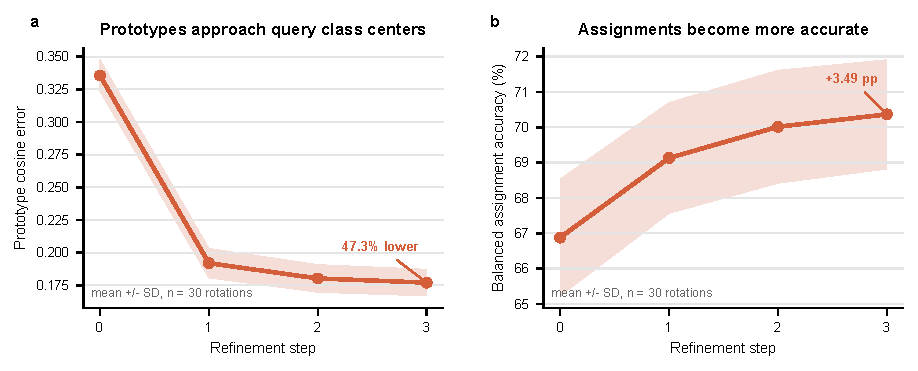
\includegraphics[width=0.82\textwidth]{figures/fig_mechanism_diagnostics.pdf}
\caption{\textbf{Prototype correction along the frozen refinement trajectory.}
\textbf{a}, Mean cosine error between the current DCTPR prototype and the true
query-class center. \textbf{b}, Balanced assignment accuracy. Curves are
mean $\pm$ descriptive standard deviation over 30 Dogs support rotations.
Query labels are used only offline for diagnosis, never as DCTPR inputs;
rotations share episode images and are not independent replicates.}
\label{fig:mechanism}
\end{figure}

Figure~\ref{fig:mechanism} traces the frozen update on the transferred Dogs
episodes. From balanced assignment at $T=0$ to the final \method assignment at
$T=3$, mean prototype cosine error relative to the true query-class center
falls from 0.336 to 0.177, a 47.3\% reduction. Balanced assignment accuracy
rises from 66.88\% to 70.36\%, a 3.49-point gain. Most of the geometric
correction occurs in the first update and the remaining steps provide smaller
increments, supporting a short fixed schedule. This diagnostic isolates the
intended prototype-correction mechanism; it does not use query labels during
inference or establish semantic complementarity between the two encoders.

\FloatBarrier
\subsection{Low-latency state-of-the-art comparison}

Table~\ref{tab:main} compares established transductive solvers using the same
features and episodes. On CUB, TIM-ADM is the most accurate method at 76.19\%.
\method reaches 74.85\%, a deficit of 1.35 points, but takes 33.3 ms rather
than 126.3 ms per rotation, a 3.8-fold reduction. \method also exceeds both MAP
arms and the LaplacianShot variants on CUB.

On Dogs, MAP-RAW is strongest overall at 70.97\%, while \method reaches
70.36\%. The 0.61-point difference is accompanied by a substantial runtime difference:
34.1 ms for \method and 1,678.6 ms for MAP-RAW, or approximately 49-fold.
\method is also 0.36 points above TIM-ADM on Dogs while remaining about four
times faster. Taking 50 ms per rotation as the low-latency task-head budget,
\method is the highest-accuracy matched solver on both CUB and Dogs (74.85\%
and 70.36\%, respectively). This is the paper's scoped low-latency
state-of-the-art result; the unrestricted accuracy leader remains TIM-ADM on
CUB and MAP-RAW on Dogs.

\begin{table}[!htbp]
\centering
\caption{Matched transductive comparison. Accuracy is the mean balanced
accuracy across three episodes and 30 rotations per dataset. Runtime is mean
milliseconds per rotation for the transductive head only. Bold marks the best
accuracy overall; underlining marks \method; $\dagger$ marks the best accuracy
under the 50-ms-per-rotation budget.}
\label{tab:main}
\begin{tabular}{lrrrr}
\toprule
& \multicolumn{2}{c}{CUB, 200-way} & \multicolumn{2}{c}{Stanford Dogs, 120-way} \\
\cmidrule(lr){2-3}\cmidrule(lr){4-5}
Method & Accuracy (\%) & Runtime (ms) & Accuracy (\%) & Runtime (ms) \\
\midrule
BL nearest support & 68.17 & 0.0 & 64.09 & 0.0 \\
BL balanced assignment & 73.50 & 10.9 & 66.88 & 12.0 \\
LaplacianShot & 68.30 & 2.2 & 64.43 & 3.9 \\
MAP-RAW & 74.30 & 1,612.9 & \textbf{70.97} & 1,678.6 \\
Signed PT-MAP adaptation & 74.37 & 1,612.5 & 70.94 & 1,666.0 \\
TIM-ADM & \textbf{76.19} & 126.3 & 70.01 & 139.2 \\
\underline{\method} & \underline{74.85}\textsuperscript{\(\dagger\)} & \underline{33.3} & \underline{70.36}\textsuperscript{\(\dagger\)} & \underline{34.1} \\
\bottomrule
\end{tabular}
\end{table}

\subsection{Locked official-test audit}
\label{sec:officialtest}

The locked audit checks whether the train-only story survives a disjoint
official-test draw without changing the method. On CUB, \method reaches
74.64\%, improves BL-NCC by 6.69 points, and remains within 1.53 points of
TIM-ADM. On three disjoint Dogs test episodes it reaches 70.49\%, gains 6.92
points over BL-NCC, and is within 0.99 points of MAP-RAW. B/L extraction takes
42.2 seconds for the 2,000-image CUB episode and 24.7--25.1 seconds per
1,200-image Dogs episode, with 1.34~GB peak allocated GPU memory. Across the
train-only one-factor audit, $T=1,2,3,5$ spans 0.36 points on CUB and 1.47
points on Dogs; temperature is more sensitive. Full solver and sensitivity
tables are retained in the reproducibility archive. These results audit the
frozen protocol and do not create a new development set.

Figure~\ref{fig:pareto} makes the operating-point comparison explicit. Under
the 50-ms task-head budget, \method is the low-latency accuracy leader on both
datasets. On CUB,
\method lies between the inexpensive balanced assignment and the more accurate
TIM-ADM solver. It recovers
$(74.85-68.17)/(76.19-68.17)=83.3\%$ of TIM-ADM's gain over BL-NCC while using
26.4\% of its task-head runtime. On Dogs, it recovers
$(70.36-64.09)/(70.97-64.09)=91.1\%$ of MAP-RAW's gain while using 2.0\% of its
runtime. The result is therefore not merely that \method is faster than the
most accurate comparator. It retains most of that comparator's improvement
over the same inductive reference.

\begin{figure}[!htbp]
\centering
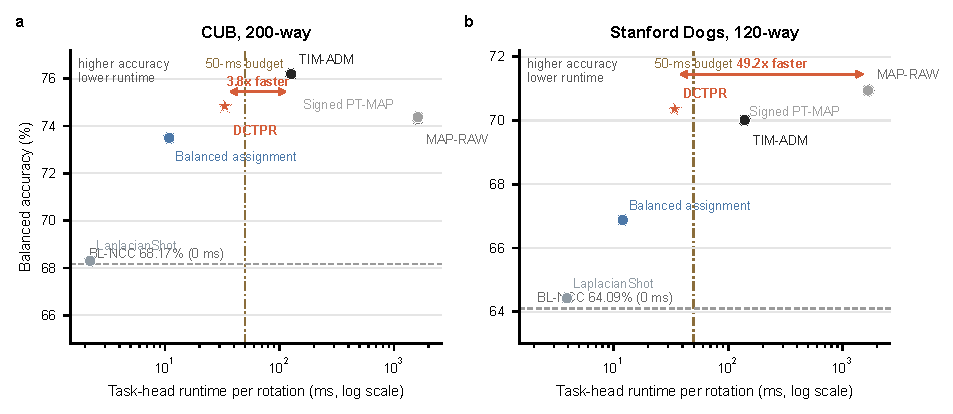
\includegraphics[width=\textwidth]{figures/fig2_accuracy_efficiency.pdf}
\caption{\textbf{Accuracy--efficiency operating points on two high-way
datasets.} \textbf{a}, CUB-200-2011, evaluated as 200-way one-shot
classification. \textbf{b}, Stanford Dogs, evaluated as 120-way one-shot
classification. Each point reports mean balanced accuracy and mean task-head
runtime across three episodes and 30 support rotations. All methods use the
same saved DINOv2 features. The dashed horizontal line is the zero-optimization
BL-NCC reference and is not assigned an artificial value on the logarithmic
runtime axis. The vertical dash-dotted line marks the 50-ms-per-rotation
task-head budget. DCTPR is 3.8 times faster than TIM-ADM on CUB and 49.2 times
faster than MAP-RAW on Dogs.}
\label{fig:pareto}
\end{figure}

\subsection{Cross-episode and cross-dataset stability}

The gain over nearest support is consistent across all six episodes
(Table~\ref{tab:robustness}a). CUB gains range from 6.59 to 6.73 points. Dogs gains
range from 5.94 to 6.58 points even though no Dogs label informed method or
baseline selection. All 30 Dogs support rotations improve over BL-NCC. The
similar gain magnitude across a bird dataset and a dog-breed dataset suggests
that the method is correcting a recurring one-shot prototype problem rather
than only exploiting one CUB episode construction.

The rotation-level view in Figure~\ref{fig:robustness}a strengthens this
descriptive result. Every one of the 60 paired rotations improves over BL-NCC,
despite different support images and disjoint episode image groups. The
dispersion is wider within episodes than the variation among episode means:
individual gains range from approximately four to nine points, whereas the six
episode means remain between 5.94 and 6.73 points. Because rotations reuse
images, these points are evidence of paired stability rather than independent
replicates for a significance test.

\begin{figure}[!htbp]
\centering

\includegraphics[width=0.82\textwidth]{figures/fig3_stability_prior.pdf}
\caption{\textbf{Stable gains and their query-prior boundary.}
\textbf{a}, DCTPR gain over BL-NCC for each support rotation; bars mark episode
means. All 60 paired differences are positive. \textbf{b}, Mean CUB macro
balanced accuracy under balanced, mild, and severe query regimes.
Uniform-prior DCTPR loses most of its balanced-task advantage under imbalance;
true counts are an oracle diagnostic only.}
\label{fig:robustness}
\end{figure}

\subsection{Query-prior stress test}
\label{sec:priorstress}

The primary protocol supplies the exact class-balanced column mass used by
Equation~\eqref{eq:marginals}. We test the consequence of violating this
assumption on CUB. In the mild regime, half the classes retain three queries and
half retain nine. In the severe regime, class counts range from one to nine.
Counts are permuted across classes with fixed seeds, and macro balanced accuracy
prevents majority classes from dominating the metric.

Table~\ref{tab:robustness}b shows that uniform-prior \method falls to 68.34\% and
68.86\%, close to nearest support and below its balanced-query result. Replacing
the uniform marginal with true class counts, solely as an oracle diagnostic,
recovers 73.35\% and 72.87\%. The 4.01--5.01 point mean gaps indicate that
incorrect class mass, rather than complete loss of query geometry, explains a
large fraction of the degradation. Oracle counts are never used as a deployable
method input.

\begin{table}[!htbp]
\centering
\caption{\textbf{Robustness checks.} \textbf{a}, Per-episode stability of the
gain over fused nearest support. \textbf{b}, CUB macro balanced accuracy under
deterministic query imbalance, averaged over three episodes. Oracle counts are
diagnostic only.}
\label{tab:robustness}
\begin{minipage}[t]{0.49\textwidth}
\centering
\small
\textbf{a}\quad Cross-episode stability\\[2pt]
\begin{tabular}{lrrr}
\toprule
Episode & BL-NCC & \method & Gain \\
\midrule
CUB E1 & 68.42 & 75.14 & +6.72 \\
CUB E2 & 68.12 & 74.71 & +6.59 \\
CUB E3 & 67.96 & 74.69 & +6.73 \\
Dogs E1 & 63.78 & 69.72 & +5.94 \\
Dogs E2 & 64.46 & 71.05 & +6.58 \\
Dogs E3 & 64.04 & 70.32 & +6.29 \\
\bottomrule
\end{tabular}
\end{minipage}\hfill
\begin{minipage}[t]{0.47\textwidth}
\centering
\small
\textbf{b}\quad Query-prior stress test\\[2pt]
\begin{tabular}{lrr}
\toprule
Method & Mild & Severe \\
\midrule
BL nearest support & 68.33 & 68.19 \\
TIM-ADM & \textbf{70.31} & 68.94 \\
\method, uniform prior & 68.34 & 68.86 \\
\method, oracle counts & 73.35 & \textbf{72.87} \\
\bottomrule
\end{tabular}\\[-1pt]
\footnotesize Mild: 3/9 queries; severe: 1--9 queries.
\end{minipage}
\end{table}

Figure~\ref{fig:robustness}b places the stress result next to the balanced
operating point. The uniform and oracle DCTPR curves coincide when the query set
is balanced because the assumed and true class marginals are identical. They
separate immediately when the class counts become non-uniform. This pattern
localizes the failure to the marginal constraint: query features still contain
recoverable information, but the uniform column mass allocates that information
to the wrong class totals.

\subsection{Class-level transfer and paired significance}
\label{sec:perclass}

Aggregate balanced accuracy can hide class-level harm, so we decompose the
development episodes by class and test the paired decisions directly. This is a
post-hoc analysis of the archived per-query predictions: it adds no inference,
no tuning, and no official-test access.

Refinement is broadly but not uniformly beneficial (Table~\ref{tab:perclass}).
On CUB, 152 of 200 classes improve, 20 are unchanged, and 28 degrade; on Dogs,
99 of 120 improve and 19 degrade. Harm is therefore not confined to a handful of
outliers, but it is shallow relative to the gain: mean harm among degraded
classes is $-3.47$ and $-2.71$ points, against mean gains of $+6.68$ and
$+6.27$ points. The worst single class loses 15.93 points on CUB and 7.78 points
on Dogs. No class collapses to zero accuracy under either method, so the update
does not sacrifice whole classes to raise the mean. The median class gain
($+4.63$ and $+5.37$ points) is below the mean, indicating a right-skewed
distribution in which a subset of poorly anchored classes contributes
disproportionately to the aggregate improvement.

Paired exact McNemar tests within each support rotation, where the query images
are distinct, confirm the direction of both comparisons. Against BL-NCC, all 60
rotations are significant at $\alpha=0.05$ and all favour \method. Against the
strongest matched solver the tests are informative in the opposite direction and
differ by dataset. On CUB, 19 of 30 rotations significantly favour TIM-ADM and
none favour \method, so the 1.35-point deficit is a real ordering rather than
noise. On Dogs, only 3 of 30 rotations reach significance, all favouring
MAP-RAW; the remaining 27 are statistically indistinguishable. The 0.61-point
Dogs deficit is thus weakly resolved at this sample size, which strengthens
rather than weakens the efficiency argument, since \method reaches that accuracy
with about 2\% of MAP-RAW's task-head runtime.

The two solvers also fail on largely the same queries. Error-set Jaccard overlap
is 0.78 on both datasets, with only 3.70\% (CUB) and 3.87\% (Dogs) of queries
misclassified by \method alone. Exclusive-error mass is therefore small and
nearly symmetric with the strongest solver's own exclusive errors. This bounds
what solver-agreement ensembling could recover in this regime and is consistent
with our own abandoned ensemble attempt, which produced a gain far below its
preregistered threshold. It also indicates that the residual errors are
dominated by shared representation-level ambiguity rather than
solver-specific behaviour.

\begin{table}[!htbp]
\centering
\caption{\textbf{Class-level transfer and paired tests} on the six development
episodes (30 support rotations per dataset). Transfer counts compare per-class
accuracy against fused nearest support. McNemar tests are two-sided exact tests
computed within single rotations and are reported as counts, not pooled, because
rotations reuse images.}
\label{tab:perclass}
\small
\begin{tabular}{@{}lrr@{}}
\toprule
Quantity & CUB (200) & Dogs (120) \\
\midrule
Positive / neutral / negative transfer & 152 / 20 / 28 & 99 / 2 / 19 \\
Mean, median class gain (pp) & +6.68, +4.63 & +6.27, +5.37 \\
Mean, worst harm among negatives (pp) & $-3.47$, $-15.93$ & $-2.71$, $-7.78$ \\
Classes at zero accuracy & 0 & 0 \\
\midrule
Strongest matched solver & TIM-ADM & MAP-RAW \\
Classes better / equal / worse & 53 / 33 / 114 & 43 / 4 / 73 \\
Rotations significant vs.\ BL-NCC, strongest & 30/30, 19/30 & 30/30, 3/30 \\
Error Jaccard; \method-only, strongest-only & 0.78; 3.70\%, 2.35\% & 0.78; 3.87\%, 3.26\% \\
\bottomrule
\end{tabular}
\end{table}

\begin{figure}[!htbp]
\centering
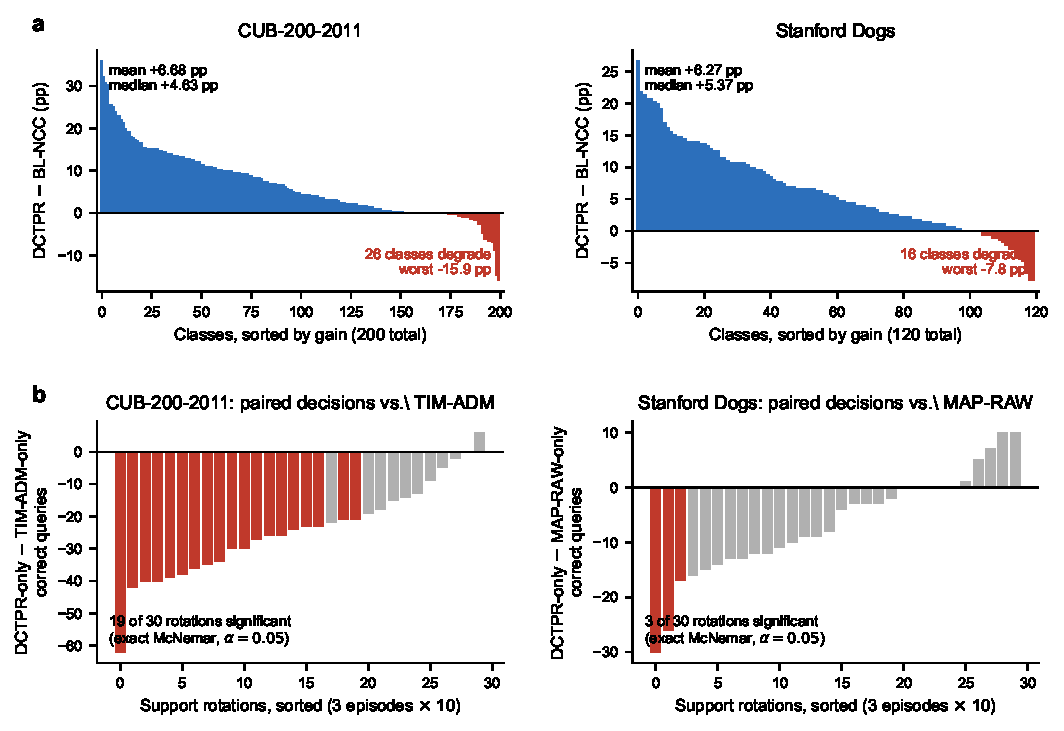
\includegraphics[width=\textwidth]{figures/fig_per_class_transfer.pdf}
\caption{\textbf{Class-level and rotation-level paired analysis.}
\textbf{a}, DCTPR minus BL-NCC balanced accuracy for each class, sorted
descending. Blue bars are positive transfer; red bars are classes that degrade.
\textbf{b}, Per-rotation difference in exclusively-correct query counts between
DCTPR and the strongest matched solver (TIM-ADM for CUB, MAP-RAW for Dogs).
Red bars reach two-sided exact McNemar significance at $\alpha=0.05$; grey bars
do not. Rotations reuse episode images and are not independent replicates.
Source data, hashes, and statistical caveats are archived in
\texttt{source\_data/per\_class\_transfer\_summary.json}.}
\label{fig:perclass}
\end{figure}

\FloatBarrier
\section{Discussion}
\label{sec:discussion}

Short support-anchored refinement recovers 83.3--91.1\% of the strongest
matched solver's improvement over nearest support. Within the 50-ms task-head
budget, it also gives the highest accuracy among the matched solvers on both
datasets, which is a scoped low-latency state-of-the-art result. Component
analysis attributes most of the correction to balanced assignment, with
dual-capacity refinement adding 1.35 points. This is not a universal Pareto
frontier beyond the tested solvers, hardware, and episodes.

TIM-ADM adds 1.35 points on CUB at 3.8 times the task-head runtime; MAP-RAW adds
0.61 points on Dogs at about 49 times the runtime. Maximum-accuracy offline use
may therefore prefer those solvers. For one uncached episode, dual-encoder
feature extraction dominates total latency. The head-level advantage matters
when features are cached or support configurations are evaluated repeatedly.
Paired rotation-level tests separate these two deficits: the CUB gap is
consistently resolved in TIM-ADM's favour, whereas 27 of 30 Dogs rotations
cannot distinguish \method from MAP-RAW. The accuracy cost of the fast head is
therefore dataset-dependent, and on Dogs it is small enough that this protocol
does not resolve it reliably.

Class-level decomposition qualifies the aggregate gain. Roughly one class in
seven is worse than nearest support, and the worst CUB class loses 15.93 points.
The gain is a favourable trade across the class distribution, not a uniform
improvement, and a deployment that cannot tolerate per-class regressions would
need a class-level safeguard that this method does not provide. The high
error-set overlap with the strongest solver further suggests the remaining
headroom lies in the frozen representation rather than in the choice of
transductive solver.

Fusion improves over both single-capacity variants on every CUB episode and
transfers to Dogs without retuning. However, it increases storage and does not
identify complementary semantic attributes; dual capacity remains an empirical
adapter choice rather than a demonstrated representation mechanism.

The balanced query prior is the main scope limitation: forcing uniform class
mass removes most of the advantage under imbalance, consistent with prior
evidence \cite{realistictransduction}. Future work should estimate proportions
without query labels and compare on public Dirichlet-imbalance protocols against
specialized methods \cite{conditionaltransport,adaptivemanifold,paddle,unem}.

Interpretation is further bounded by matched feature-level reimplementations,
image-reusing support rotations, and the known balanced query prior. The locked
official-test audit reduces, but does not remove, protocol dependence; public
imbalanced evaluation with matched backbones and multi-hardware end-to-end
latency remain future work.

\section{Conclusion}
\label{sec:conclusion}

We introduced \method, a training-free dual-capacity adapter for balanced,
high-way, one-shot fine-grained recognition. Across CUB and Stanford Dogs, it
improves fused nearest-support accuracy by 6.68 and 6.27 percentage points,
respectively. It retains 83.3--91.1\% of the strongest matched solver's gain
while using 2.0--26.4\% of that solver's task-head runtime. A locked
official-test audit preserves the same relative behavior without retuning.
Within a 50-ms task-head budget, it achieves the highest accuracy among the
matched solvers on both datasets, establishing a scoped low-latency
state-of-the-art result. These results support short, support-anchored
query-center refinement as a practical operating point when features are cached
and the query prior is balanced. Removing that prior requires a different
inference design.

\bibliography{references}
\bibliographystyle{spiebib}

\end{document}
